\documentclass{report}
\usepackage[utf8]{inputenc}
\usepackage{graphicx}
\usepackage{pdfpages}
\usepackage{amsmath}
\usepackage{hyperref}
\usepackage[document]{ragged2e}
\graphicspath{ {./images/} }

\title{IoT Methodology}
\author{Ann-Kareen Gedeus}
\date{February 2022}

\begin{document}

\maketitle

\section{Overview}
This project was designed to collect pulse sensor data from an Arduino MKR board and then send that data to the Blynk Cloud where that data would be grabbed and displayed on a Web app. Furthermore, the project specifies that users need to interact with the web app in order to change the state of the builtin LED on the device.


\section{IoT Design Methodology}
\subsection{Purpose and Requirements Specification}
\textbf{Purpose:} A pulse sensor system that monitors the BPM of users using a web application to display the data and control device led.\\
\textbf{Behavior:} The pulse sensor device should send it's data to the IoT cloud and that data needs to be displayed on the web app. Furthermore when the LED is toggled on the web app that information needs to be delivered to the cloud and the cloud will send that instruction to the Arduino device. \\
\textbf{System Management Requirement:} The system should provide BPM data and control of LED buttons. \\
\textbf{Data Analysis Requirement:} None. \\
\textbf{Application Development Requirement:} Application will live locally on device to display BPM data. \\
\textbf{Security Requirement:} Authentication token.

\begin{figure}
\subsection{Process Specification}
    \centering
    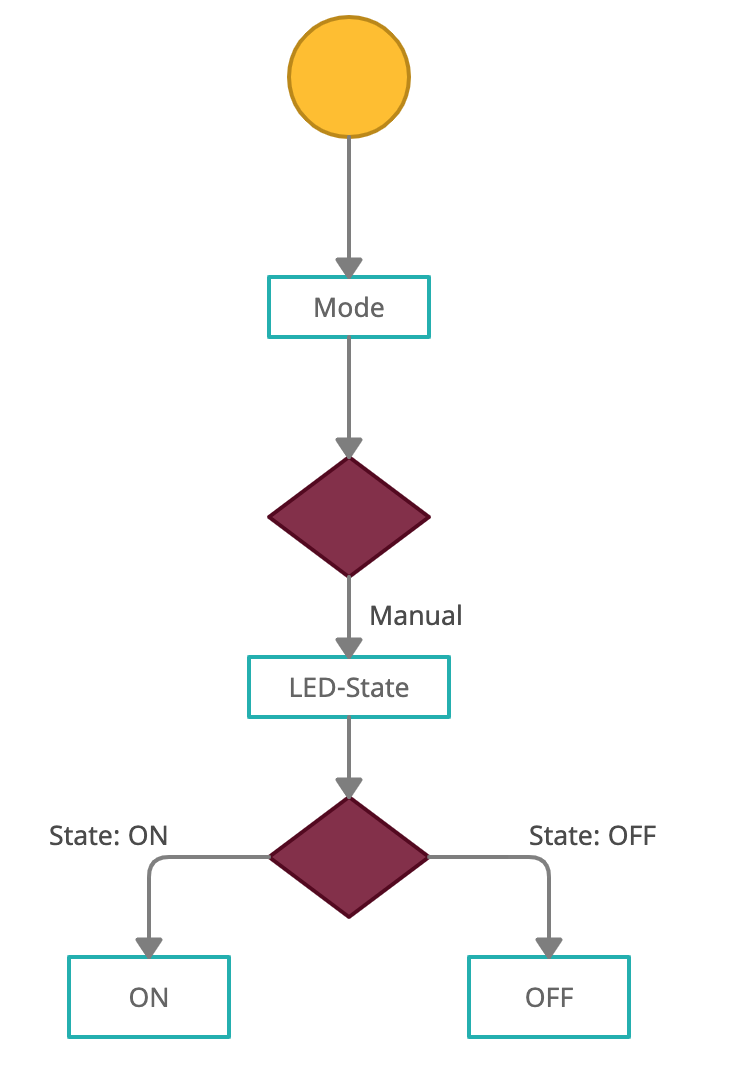
\includegraphics[scale=0.2]{images/step2.png}
    \caption{The figure above defines the state of the LED, known as the LED-State. The buttons on the web app and cloud define the led in two states: ON or OFF. The LED-State is manually changed by the user through the web app. If the user chooses the state ON the LED is turned on. If the user chooses the state OFF the LED is turned off.}
    \label{fig:image1}
\end{figure}

\begin{figure}
\subsection{Domain Model Specification}
    \centering
    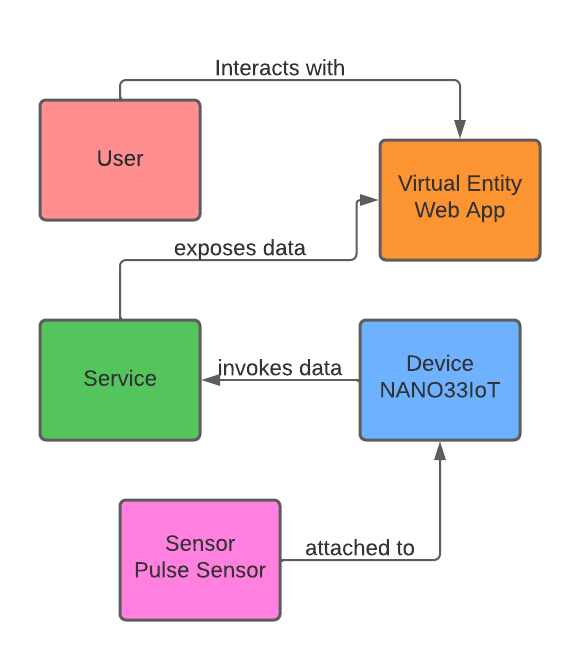
\includegraphics[scale=0.7]{images/step3(new).png}
    \caption{ The figure above defines the attributes and relationships between entities and objects. The first relationship is between the user and the virtual entity. In this relationship, the user interacts with the web app either to view the pulse sensor data or to control the led. The second relationship is between the service (Blynk Cloud) and the web app, the service exposes the data (pulse sensor data) from its platform to the web app. The third relationship is between the cloud service and the device, this relationship allows for the service to invoke and get data from the physical device. The lat relationship is between the sensor and the device. In this relationship, the sensor is attached to the device and creates the conditions for data creation.}
    \label{fig:image2}
\end{figure}

\begin{figure}
\subsection{Information Model Specification}
    \centering
    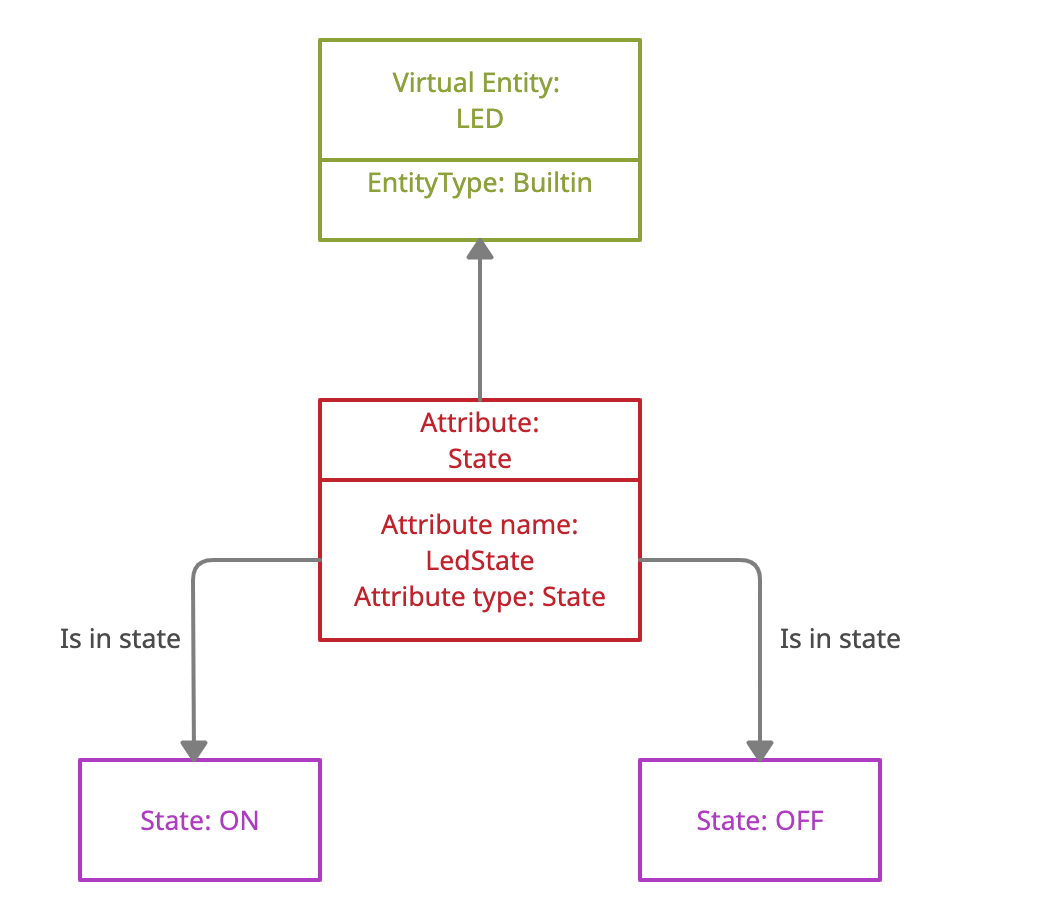
\includegraphics[scale=0.2]{images/step4.png}
    \caption{ In the figure above the relations and attributes of the virtual entity are defined. The virtual entity defined is the LED and the attributed state given to the led is LEDState on the web app. This state has two components which are the ON or OFF state.}
    \label{fig:image3}
\end{figure}

\begin{figure}
\subsection{Service Specifications}
    \centering
    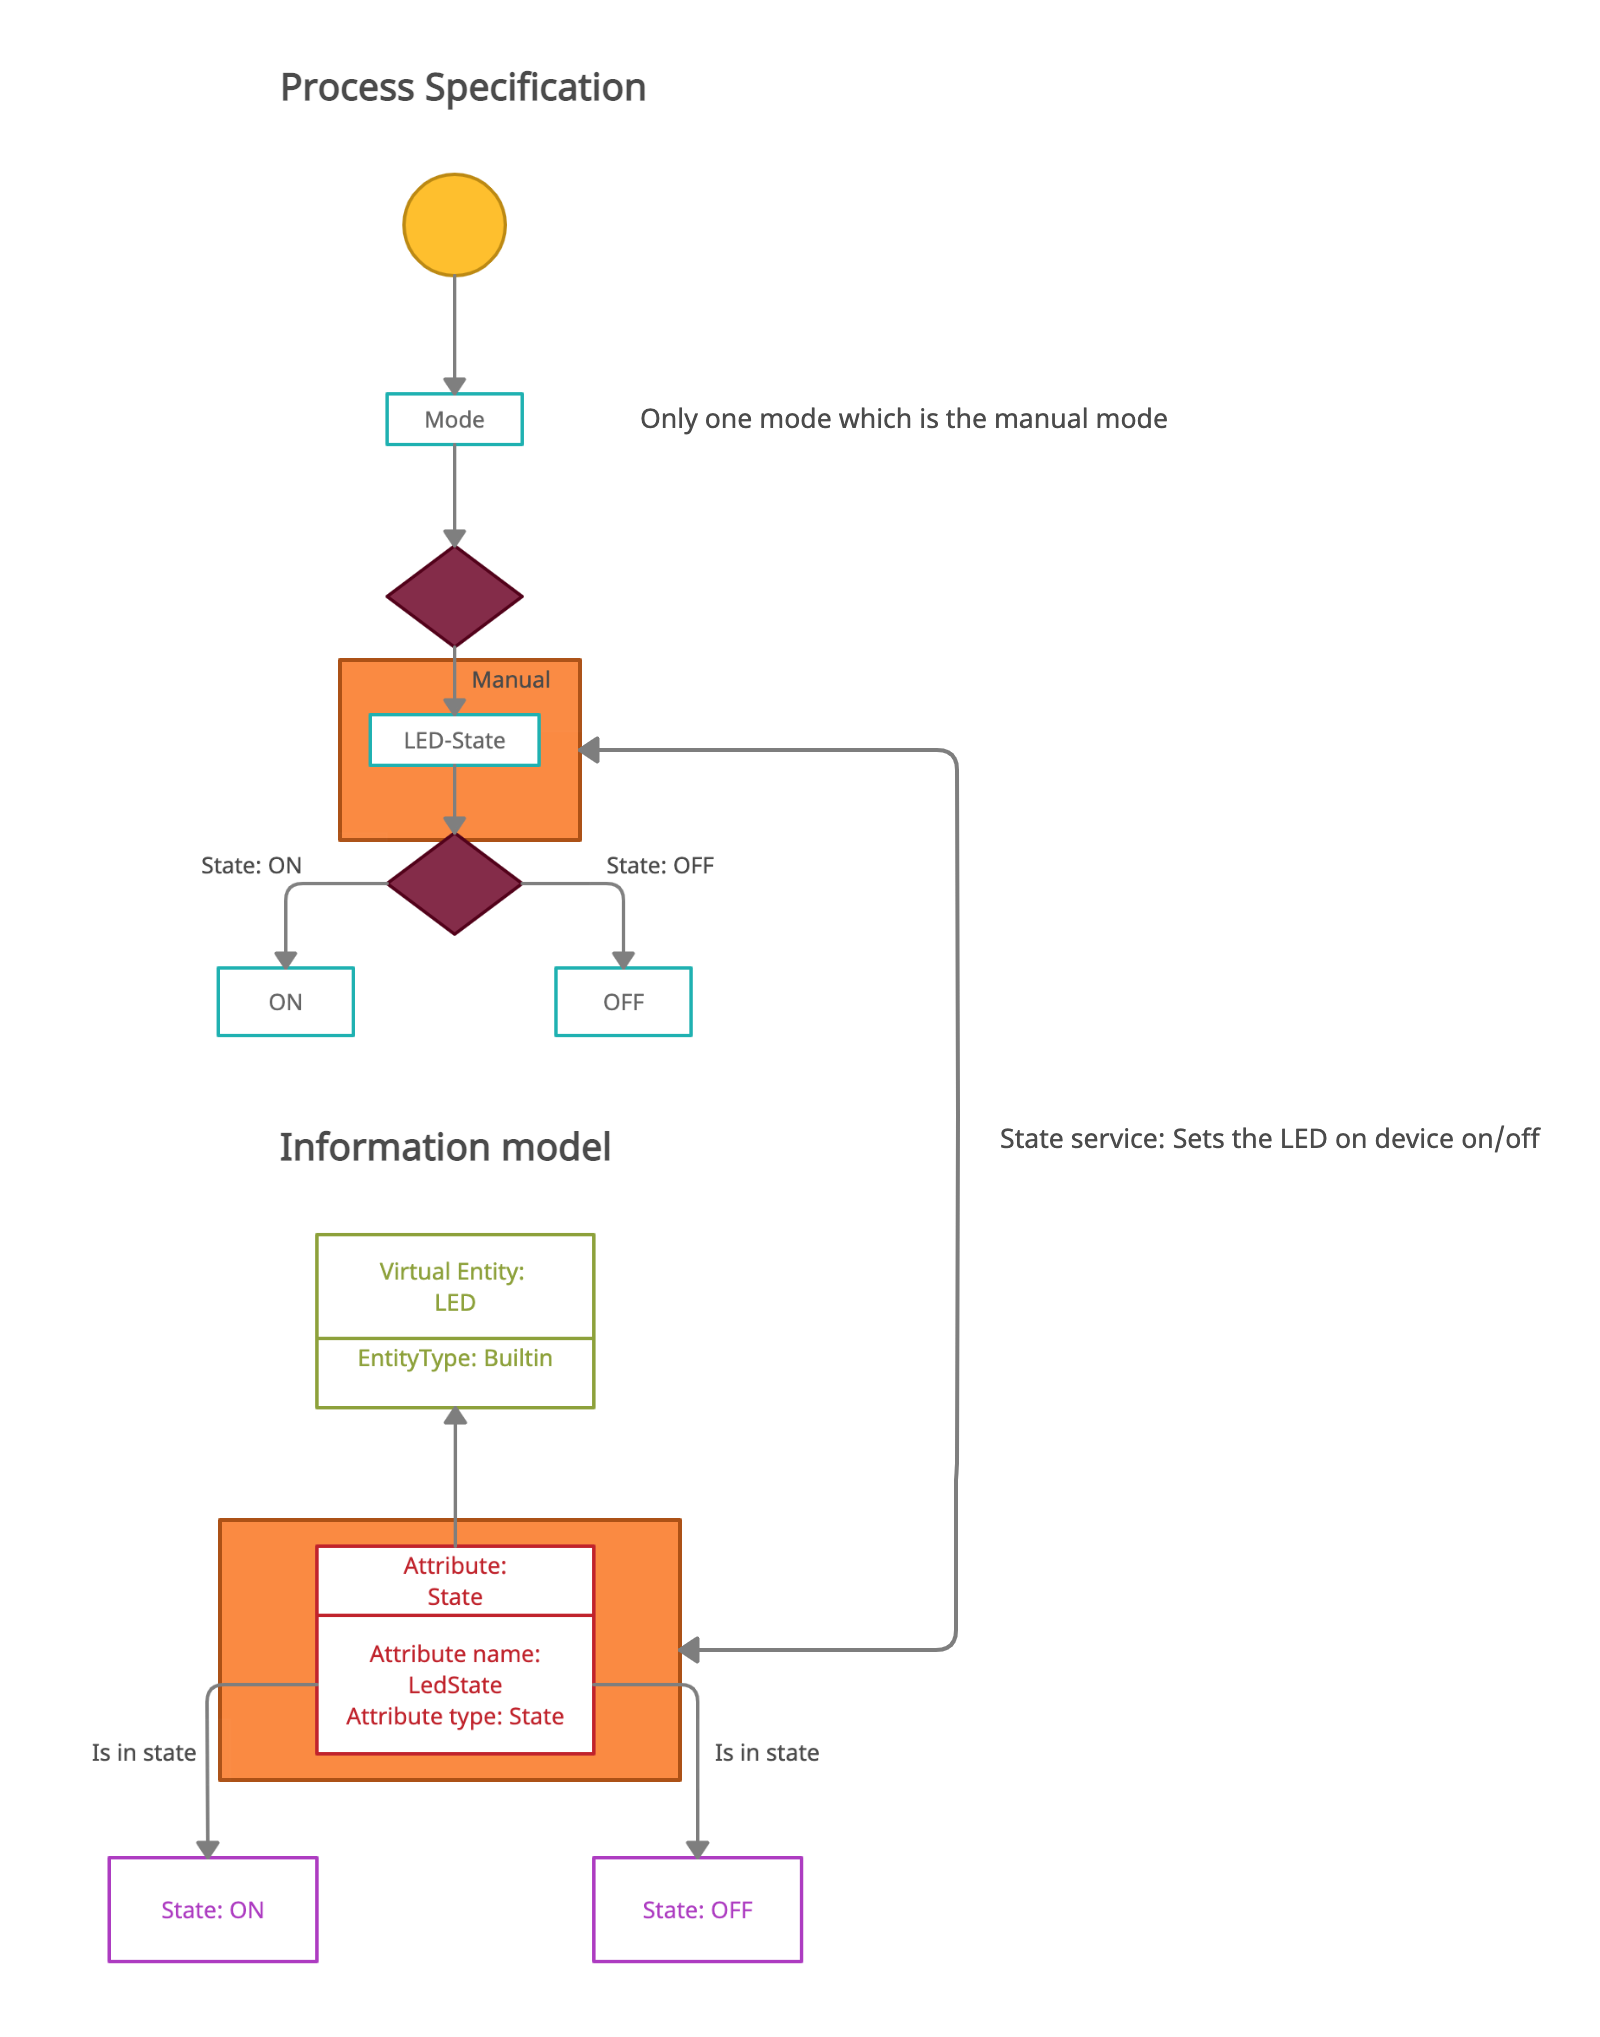
\includegraphics[scale=0.1]{images/step5.png}
    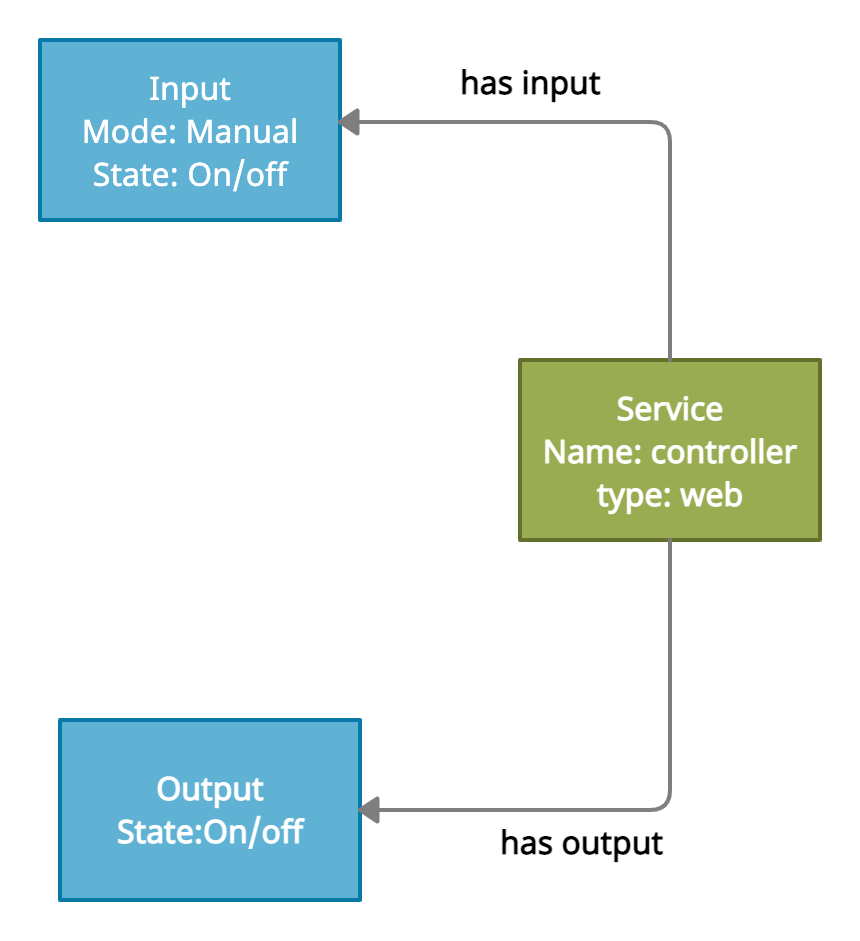
\includegraphics[scale=0.2]{images/step5 (1).png}
    \caption{In the figure above the fifth step of the IoT design methodology is defined for our service specifications. The only service here is the led control on the web app. The service checks if the led has an input and output of ON or OFF.}
    \label{fig:image4}
\end{figure}

\begin{figure}
\subsection{IoT level Specification}
    \centering
    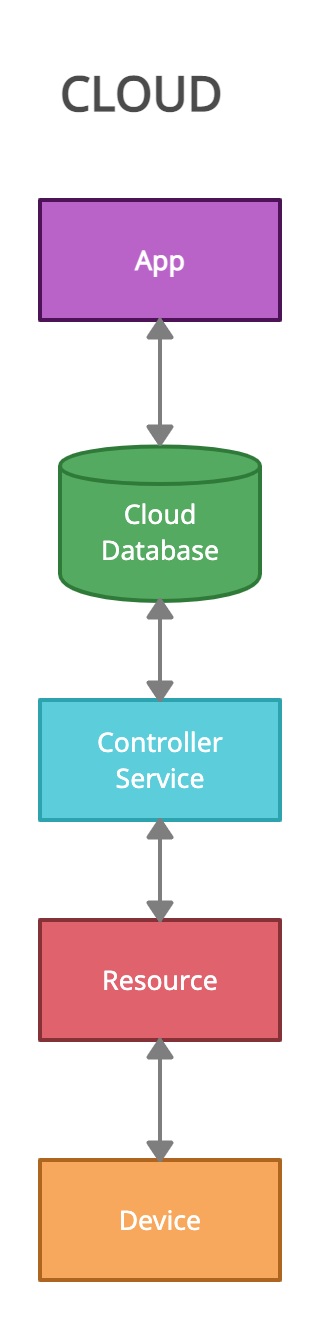
\includegraphics[scale=0.2]{images/step6.png}
    \caption{The IoT level is defined above. Our IoT level system only needs a cloud component. In this cloud level the app (web app) interacts with the cloud (Blynk Cloud) to send LEDState data and the cloud interacts with the app to send sensor data. This is connected to the controller service (Arduino IDE) which is connected to the resource (Internet, Memory, Processing) and ultimately the device.}
    \label{fig:image5}
\end{figure}

\begin{figure}
\subsection{Functional View Specification}
    \centering
    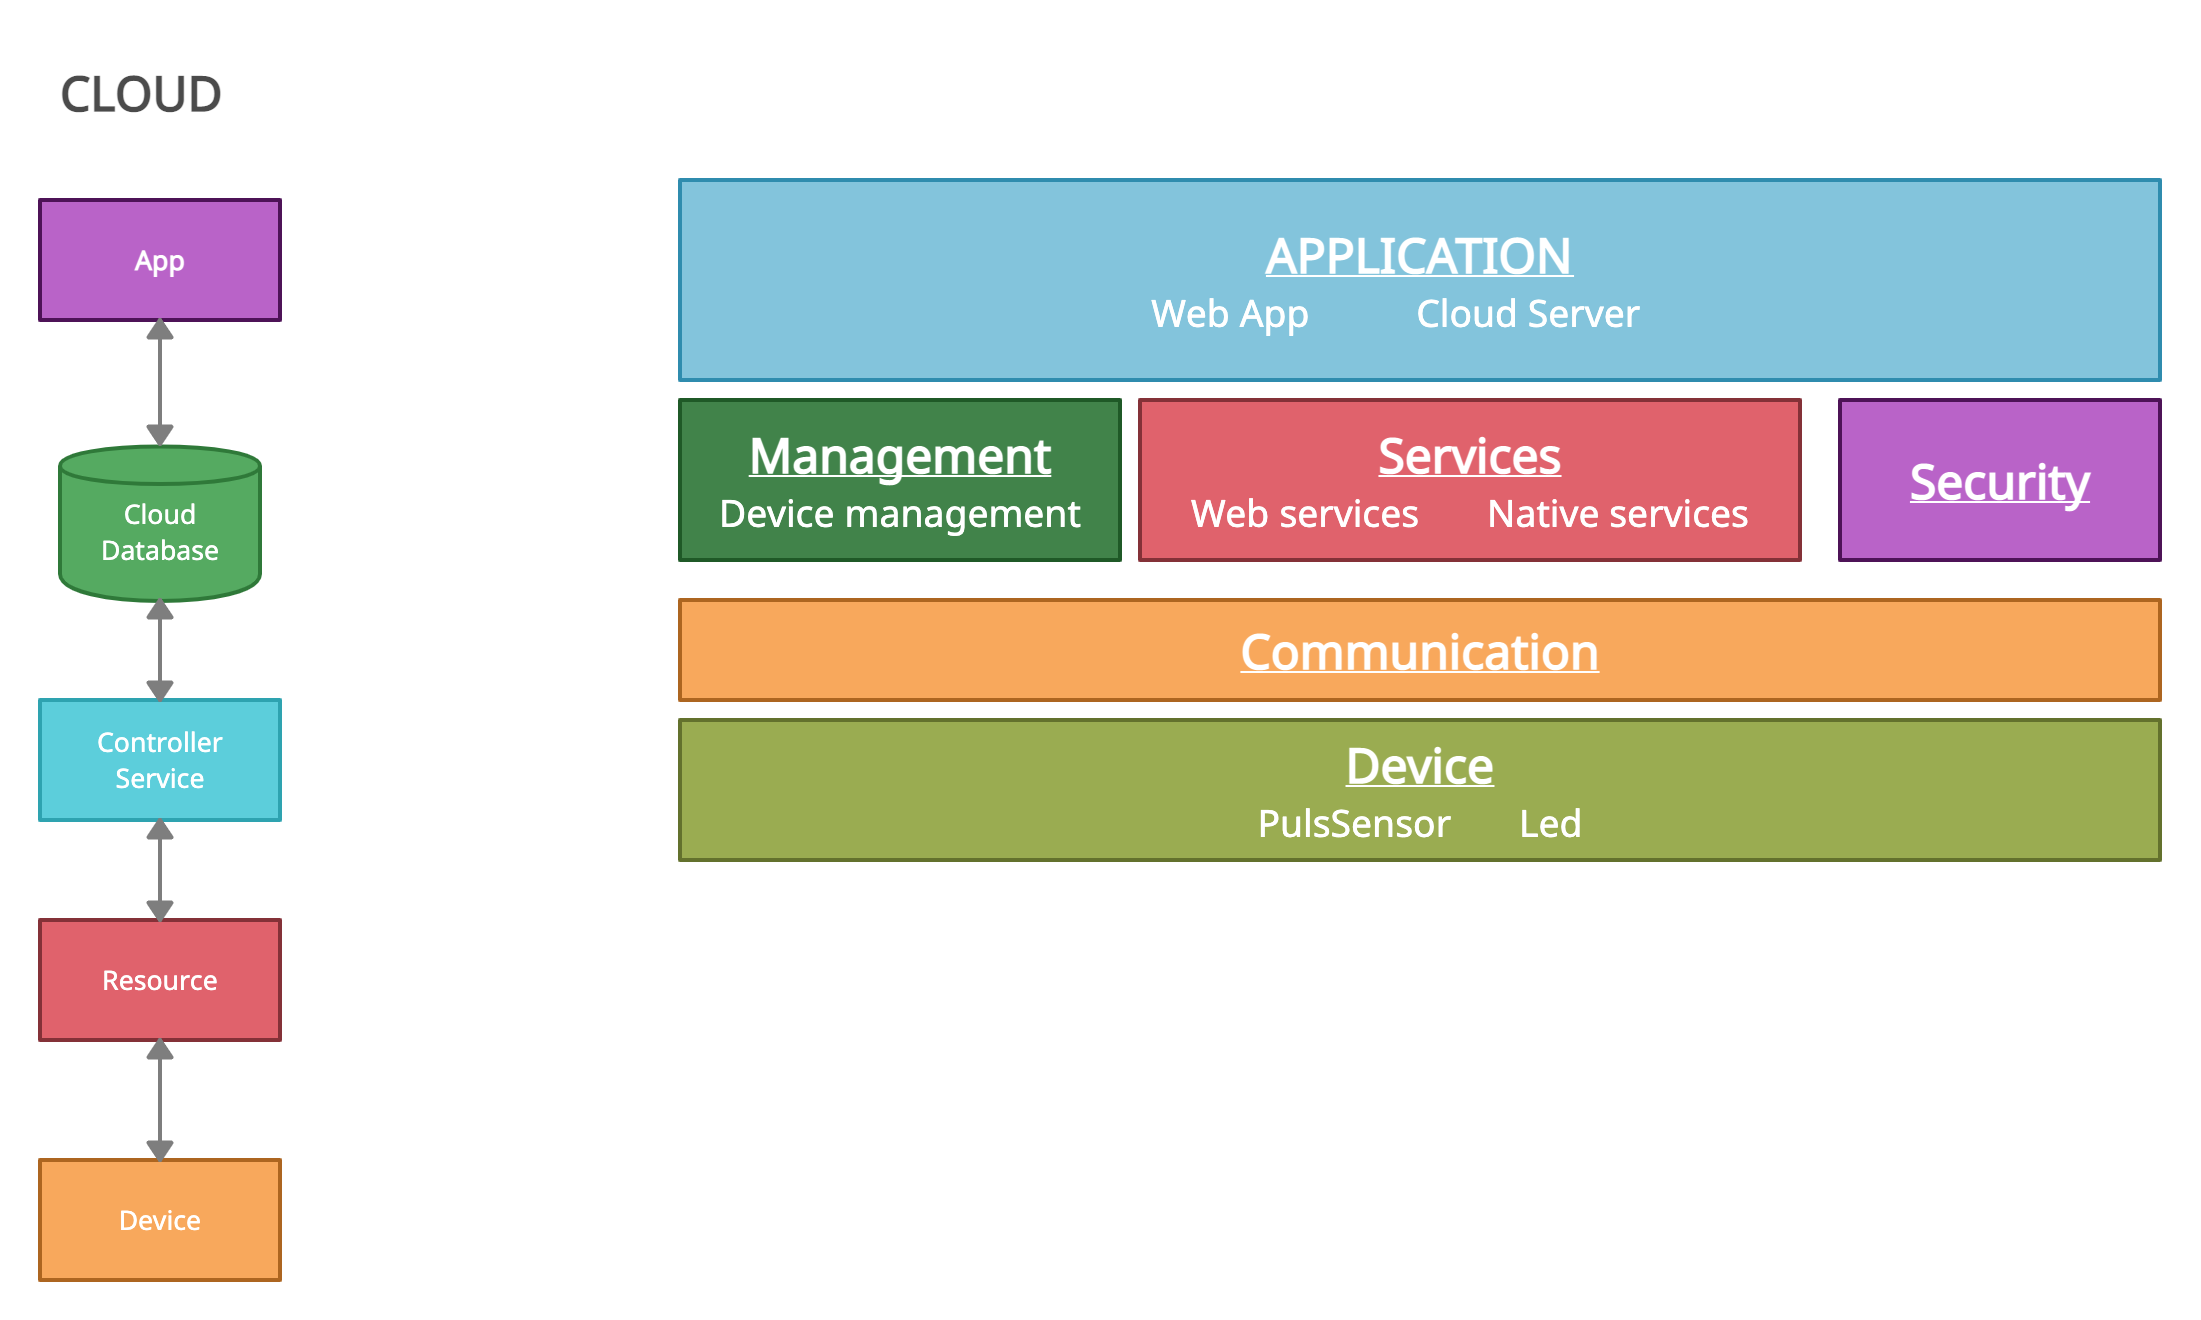
\includegraphics[scale=0.15]{images/step7.png}
    \caption{Defines the functions of the IoT systems grouped into various functional groups}
    \begin{itemize}
    \item IoT Device maps to device functional group and to management functional group
    \item Resources maps to device and communication functional group
    \item Controller service maps to native services functional group and cloud database maps to web services functional group
    \item Cloud database maps to management functional group
    \item App maps to application, management, and security functional groups
\end{itemize}
    \label{fig:image6}
\end{figure}

\begin{figure}
\subsection{Operational View Specification}
    \centering
    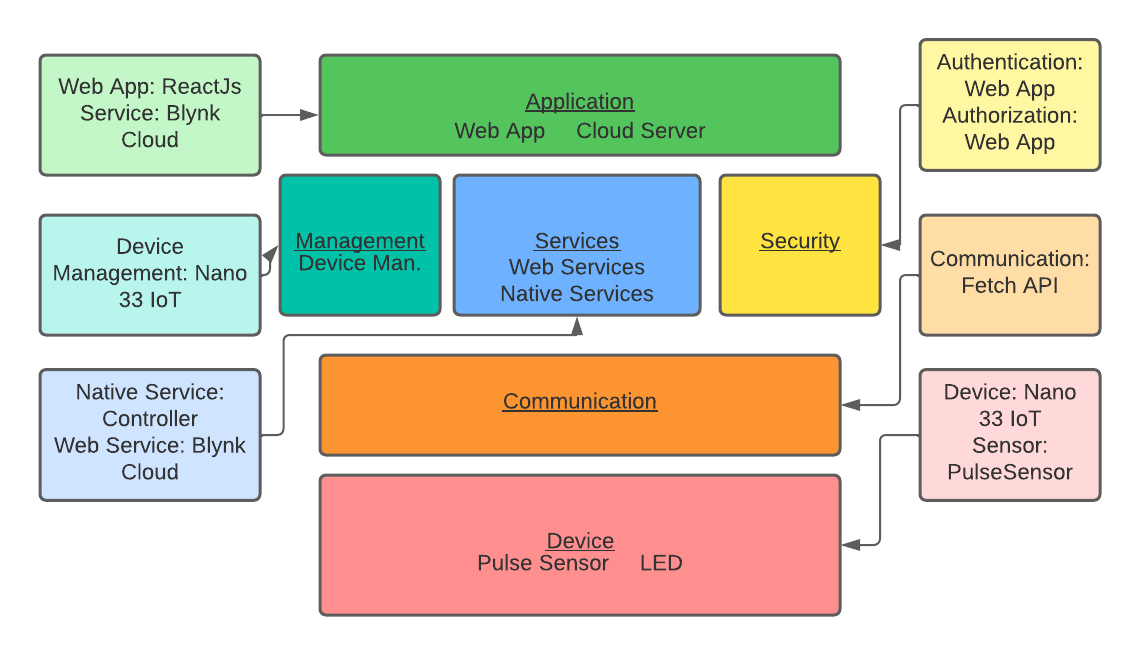
\includegraphics[scale=0.6]{images/Step8.png}
    \caption{Elements of the IoT system are defined}
    \label{fig:image7}
\end{figure}

\begin{figure}
\subsection{Device Component Integration}
    \centering
    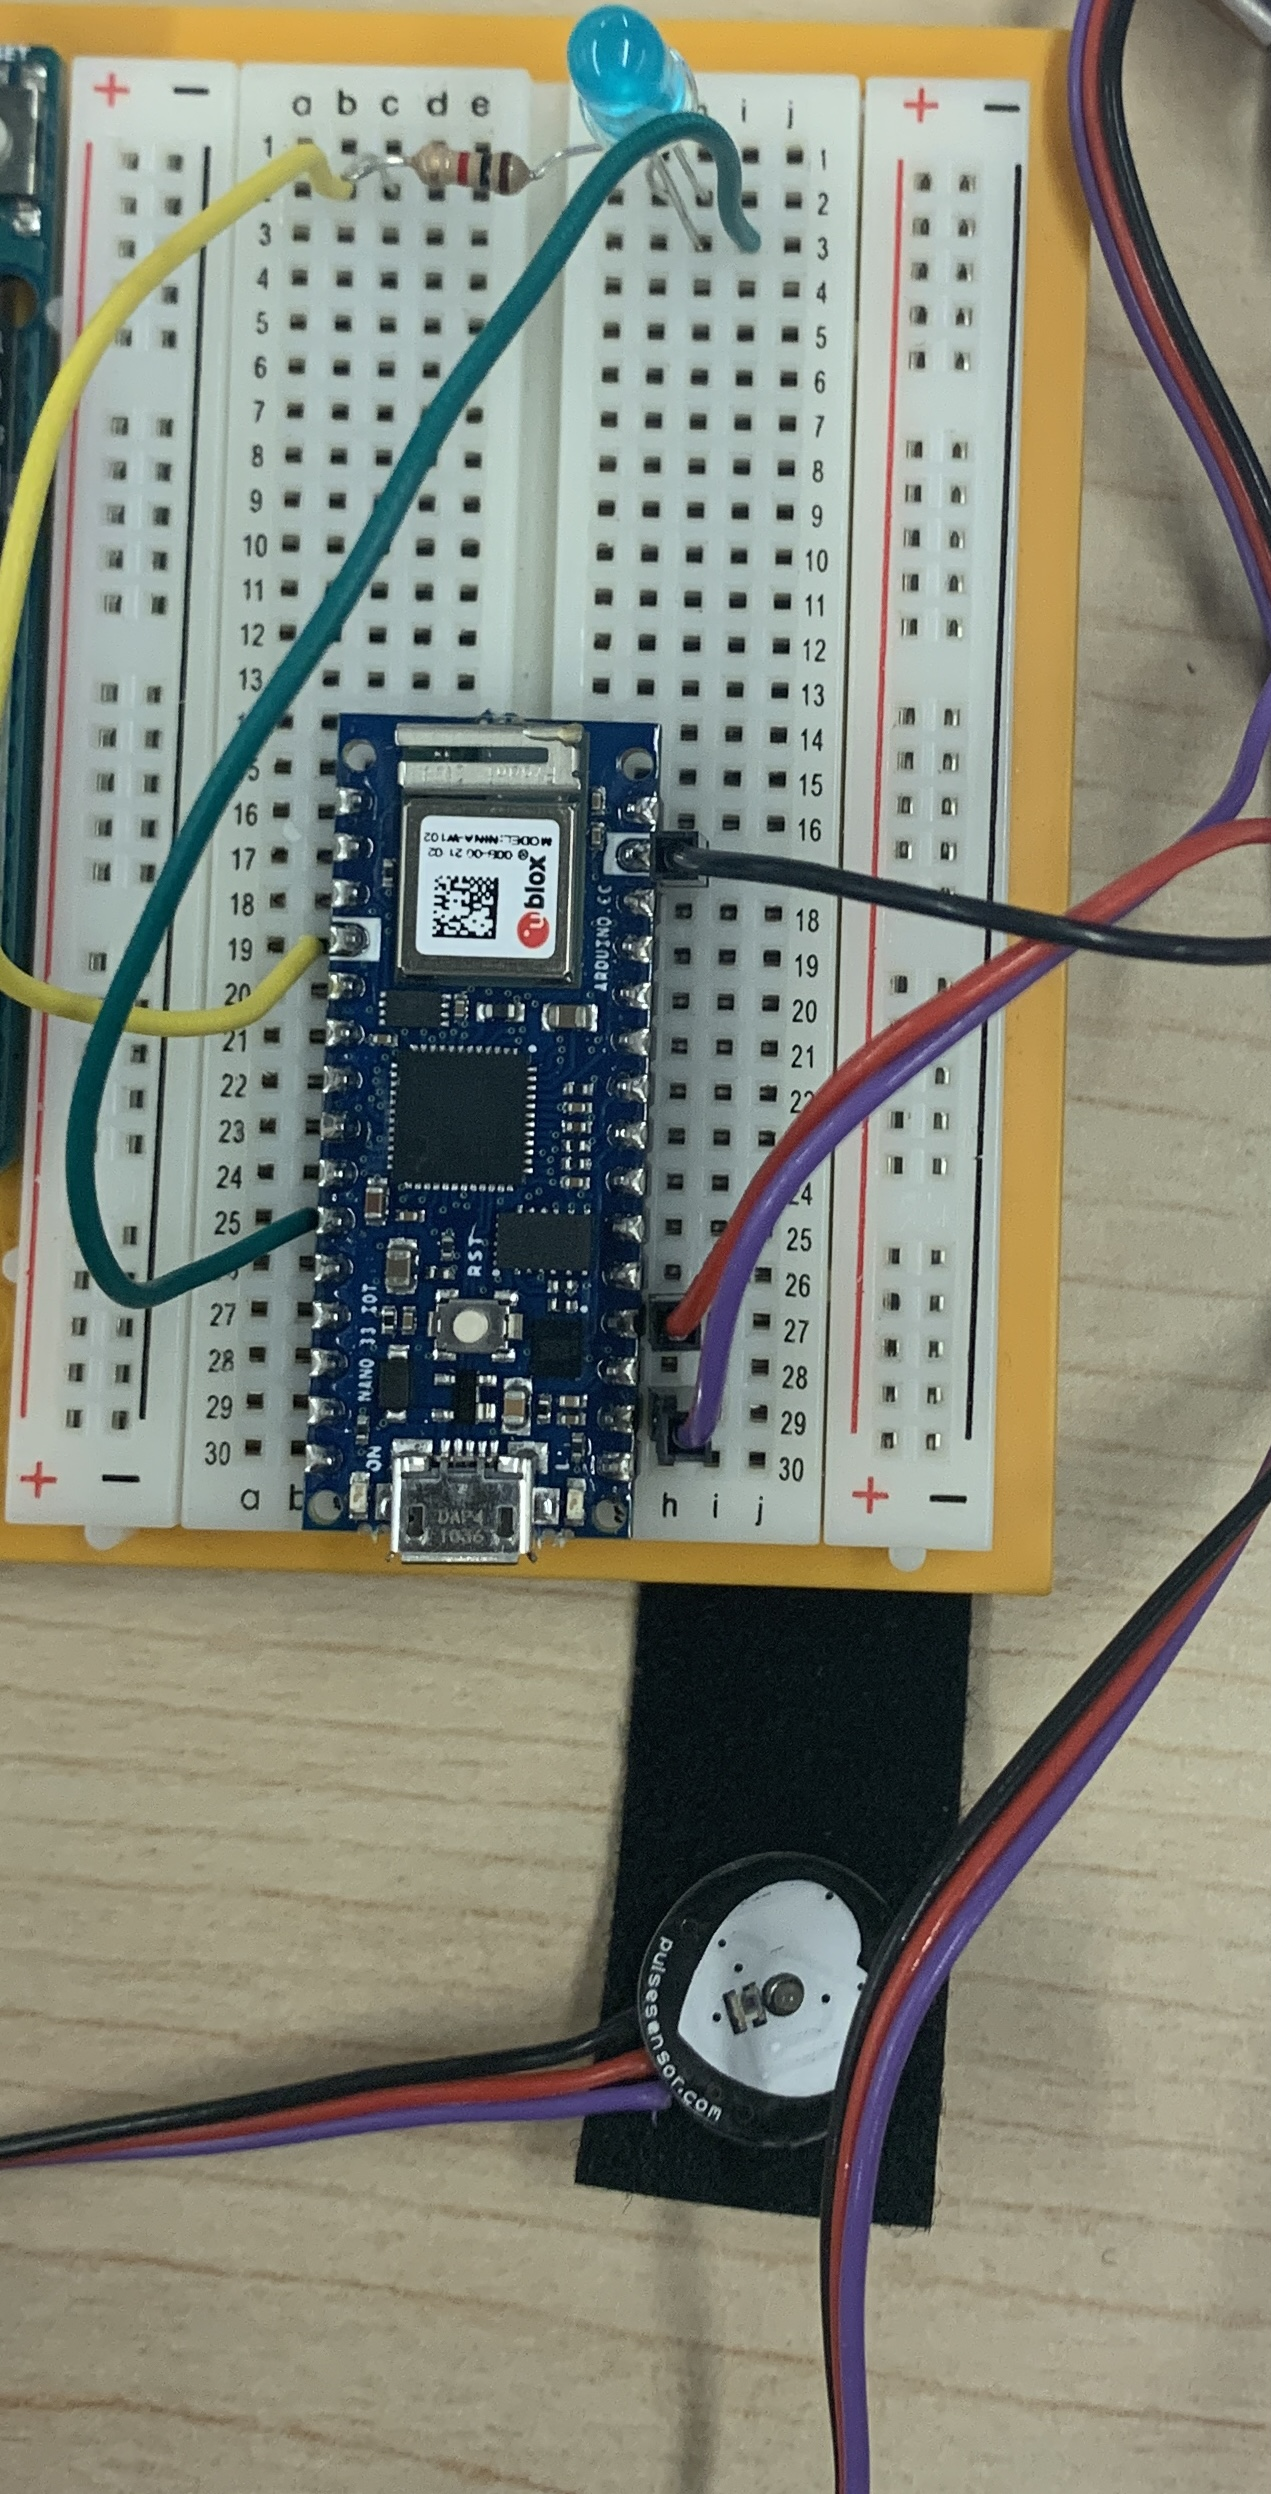
\includegraphics[scale=0.10]{images/device.JPG}
    \caption{Device Component Integration}
    \label{fig:image8}
\end{figure}


\begin{figure}
\subsection{Application Development}
    \centering
    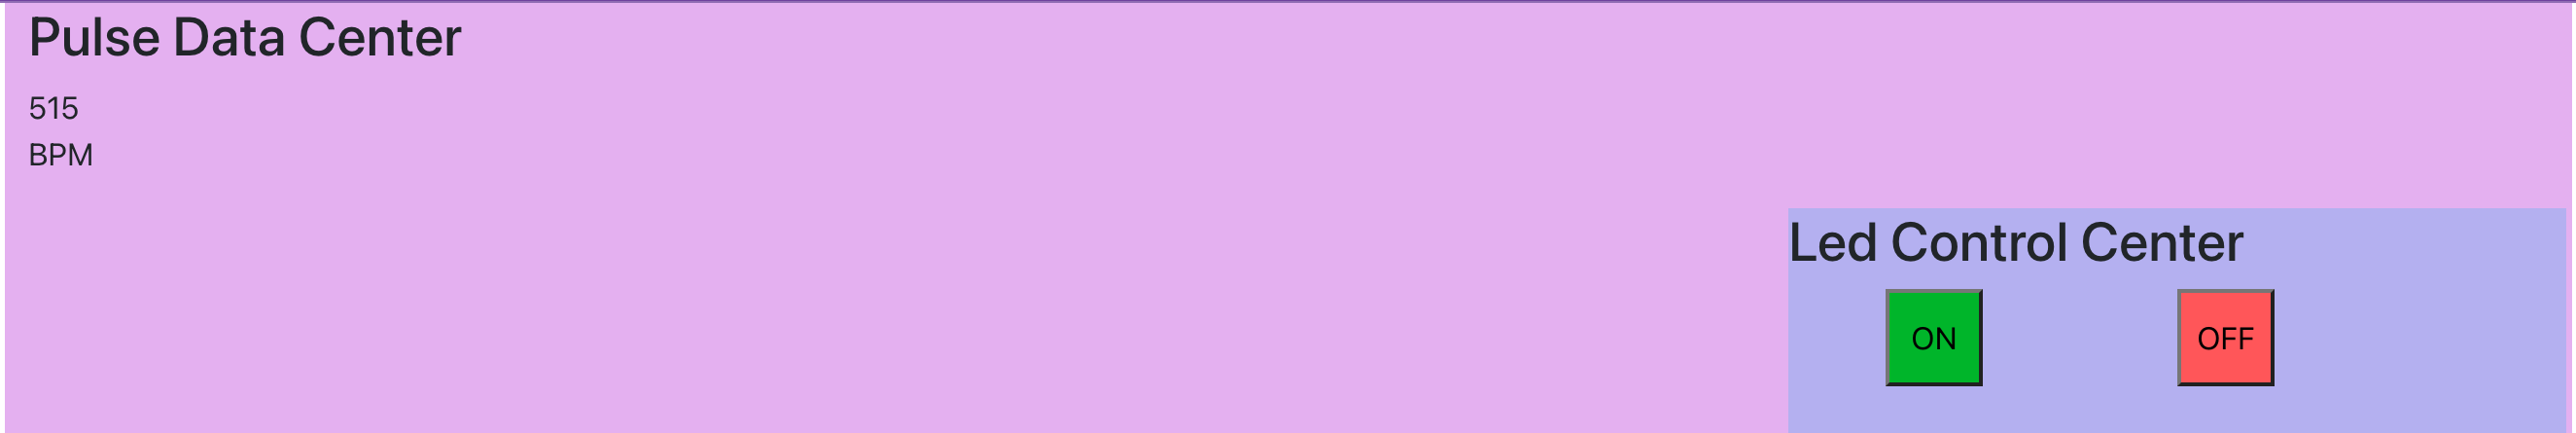
\includegraphics[scale=0.3]{images/AppDisplay.png}
    \caption{Web Application using ReactJs and BootStrap}
    \label{fig:image9}
\end{figure}


\section{Schematic}
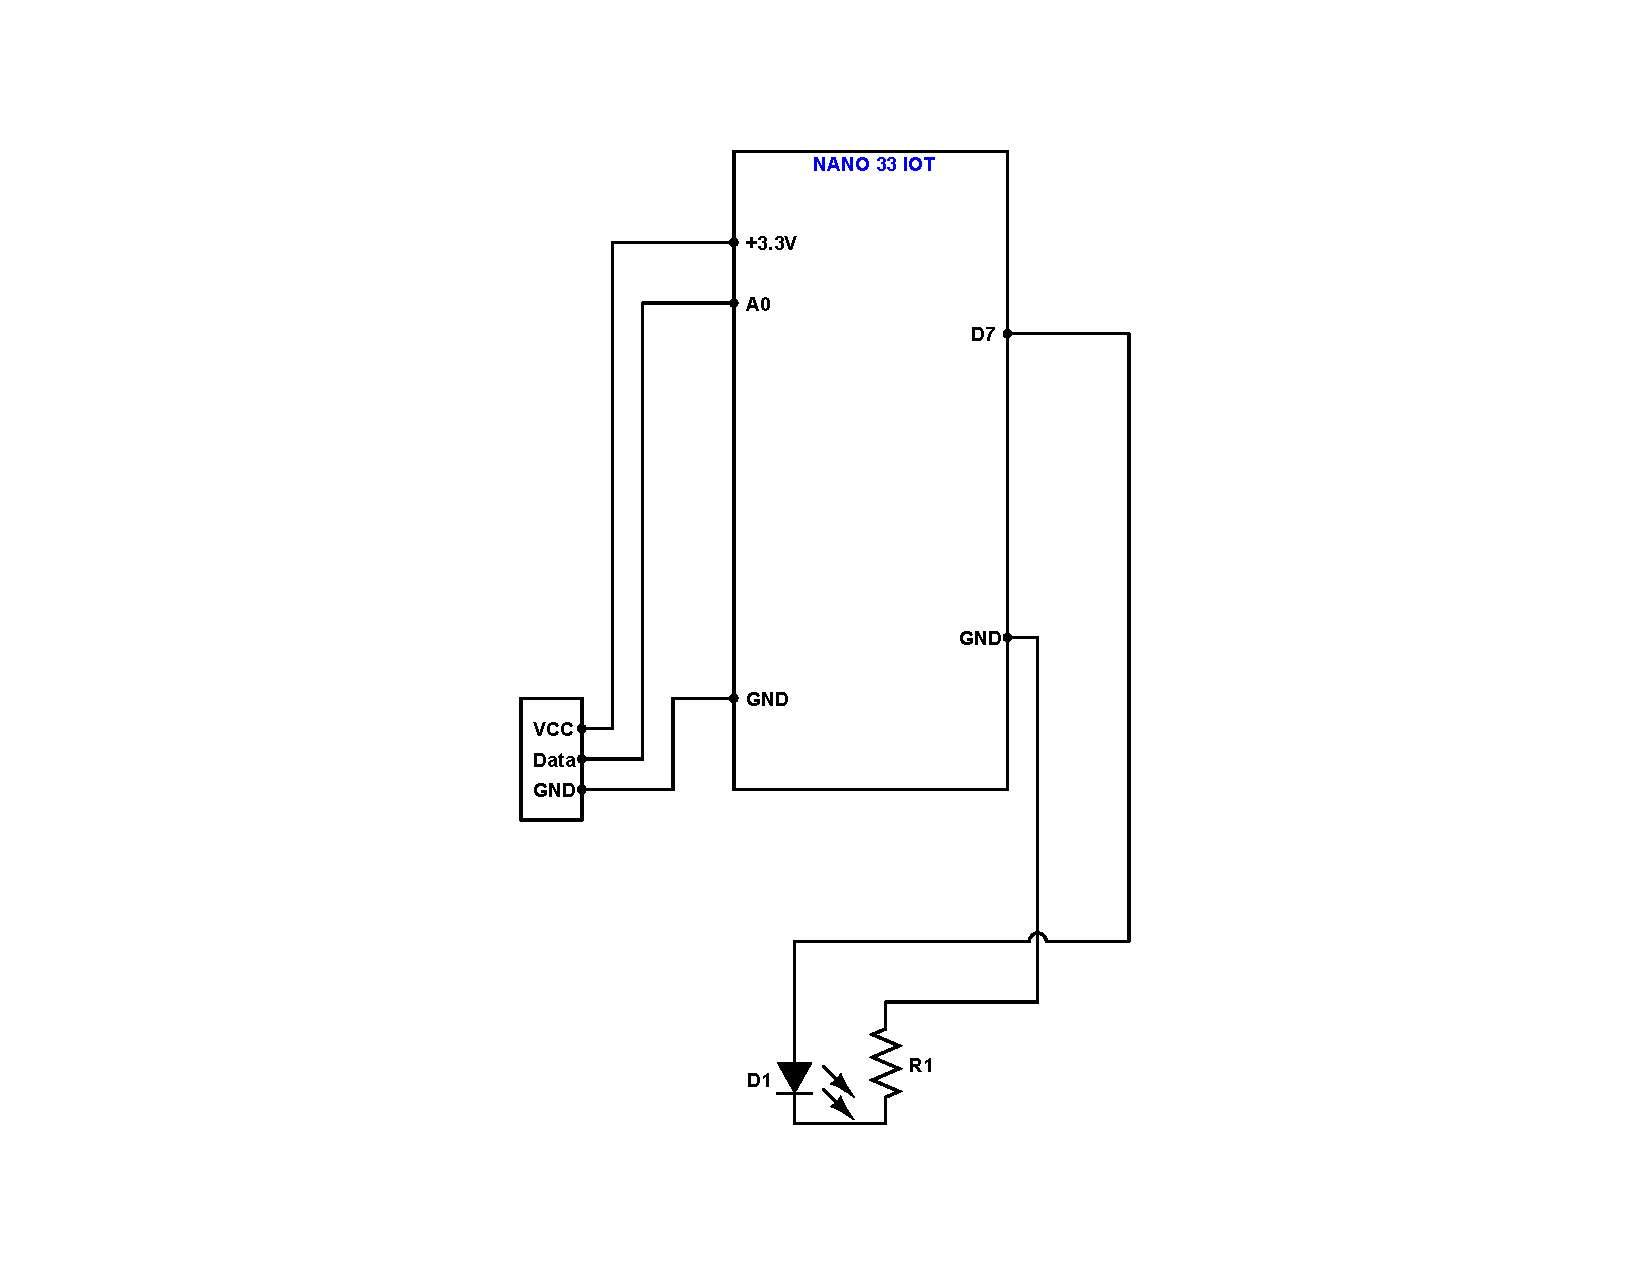
\includegraphics[scale=0.5]{documents/schematicsNano.pdf}
\centering
\caption{Figure 10: Circuit of Led and Pulse sensor}
\label{fig:image10}

\raggedright
\section{Bill of Materials}
\begin{center}
\begin{tabular}{||c c c c c||} 
 \hline
 Bom Level & Part Number & Part Name & Description & Quantity \\ [0.5ex] 
 \hline\hline
 1 & 0-100 & Nano 33 Iot & Arduino Device & 1 \\ 
 \hline
 1 & 0-101 & Pulse Sensor & Sensor & 1 \\
 \hline
 1 & 0-102 & Arduino IDE & Software & 1 \\
 \hline
 1 & 0-103 & Blynk Cloud & Software & 1 \\
 \hline
 2 & 0-104 & Web App (ReactJs) & Software & 1 \\
 \hline
 2 & 0-105 & Led & Hardware & 1 \\
 \hline
 2 & 0-106 & Resistor & Hardware & 1 \\
 \hline
 2 & 0-107 & Wire & Hardware & 2 \\ [1ex] 
 \hline
\end{tabular}
\end{center}

 

\raggedright
\section{References}
\begin{enumerate}
  \item \href{https://docs.blynk.io/en/blynk.cloud/https-api-overview}{Blynk API Documentation}
  \item \href{ https://create.arduino.cc/projecthub/rocketman27/led-blink-with-blynk-2-0-e86daa}{LED Blynk Code}
  \item \href{https://docs.blynk.io/en/legacy-platform/legacy-articles/how-to-display-any-sensor-data-in-blynk-app}{Blynk Sensor Code} 
  \item \href{https://www.youtube.com/watch?v=E8uka5CjLKw}{REST API}
  \item \href{ https://www.youtube.com/watch?v=SPM4xyYd9MI}{Fetch API for beginners}
  \item \href{ https://www.youtube.com/watch?v=E0UGGxd2DOo}{Real-time data with Fetch API}
  \item \href{https://www.youtube.com/watch?v=T3Px88x_PsA}{Fetch API with ReactJs}
\end{enumerate}


\end{document}
